% =====================================================================
%  ANLP Assignment 1 -- Transformers from Scratch, Architectural
%  Variants, and Byte Latent Transformers
%
%  Formatting follows the brief: 12pt Times New Roman, 1-inch margins,
%  max 6 pages excluding references and links.
%
%  Compile on Overleaf with pdfLaTeX:
%     Report.tex -> (bibtex) -> Report.tex -> Report.tex
% =====================================================================
\documentclass[12pt,a4paper]{article}

\usepackage[margin=1in]{geometry}
\usepackage{amsmath}                  % must precede newtxmath
\usepackage{newtxtext,newtxmath}      % Times New Roman text + matching math
                                      % (newtxmath supplies the AMS symbols, so
                                      %  amssymb must NOT be loaded -- it clashes
                                      %  on \Bbbk)
\usepackage{booktabs}
\usepackage{graphicx}
\usepackage{subcaption}
\usepackage{multirow}
\usepackage[numbers,sort&compress]{natbib}
\usepackage[hidelinks,breaklinks]{hyperref}
\usepackage{url}
\usepackage{microtype}

\graphicspath{{figures/}}

% Tighter float spacing so the six-page budget is achievable
\setlength{\textfloatsep}{7pt plus 2pt minus 2pt}
\setlength{\intextsep}{7pt plus 2pt minus 2pt}
\setlength{\abovecaptionskip}{3pt}
\setlength{\belowcaptionskip}{0pt}

\newcommand{\cfg}[1]{\textbf{#1}}

% Numbers generated from outputs/all_results.json by:
%     python report/make_tables.py
% results_macros.tex holds only \newcommand definitions (preamble-safe);
% the table environments themselves are \input inside Section 5.
% Auto-generated by report/make_tables.py -- do not edit by hand.
% Inline single-number macros, e.g. \CfgOneBit, \CfgFiveMem.
\newcommand{\CfgOneBit}{97.17}
\newcommand{\CfgOneSeq}{77.20}
\newcommand{\CfgOneLev}{0.44}
\newcommand{\CfgOnePar}{7.62}
\newcommand{\CfgOneSec}{143.0}
\newcommand{\CfgOneMem}{372}
\newcommand{\CfgOnePpl}{1.19}
\newcommand{\CfgOneGen}{6.6}
\newcommand{\CfgOneTok}{96.98}
\newcommand{\CfgOneEp}{25}
\newcommand{\CfgOneLoss}{0.1747}
\newcommand{\CfgOneBleu}{90.34}
\newcommand{\CfgOneRouge}{95.10}
\newcommand{\CfgOneEpochs}{25}
\newcommand{\CfgTwoBit}{97.61}
\newcommand{\CfgTwoSeq}{81.20}
\newcommand{\CfgTwoLev}{0.35}
\newcommand{\CfgTwoPar}{7.62}
\newcommand{\CfgTwoSec}{153.8}
\newcommand{\CfgTwoMem}{372}
\newcommand{\CfgTwoPpl}{1.16}
\newcommand{\CfgTwoGen}{6.6}
\newcommand{\CfgTwoTok}{97.52}
\newcommand{\CfgTwoEp}{24}
\newcommand{\CfgTwoLoss}{0.1468}
\newcommand{\CfgTwoBleu}{92.27}
\newcommand{\CfgTwoRouge}{96.06}
\newcommand{\CfgTwoEpochs}{25}
\newcommand{\CfgThreeBit}{96.81}
\newcommand{\CfgThreeSeq}{73.80}
\newcommand{\CfgThreeLev}{0.54}
\newcommand{\CfgThreePar}{6.73}
\newcommand{\CfgThreeSec}{147.2}
\newcommand{\CfgThreeMem}{360}
\newcommand{\CfgThreePpl}{1.20}
\newcommand{\CfgThreeGen}{6.1}
\newcommand{\CfgThreeTok}{96.57}
\newcommand{\CfgThreeEp}{25}
\newcommand{\CfgThreeLoss}{0.1847}
\newcommand{\CfgThreeBleu}{88.54}
\newcommand{\CfgThreeRouge}{94.21}
\newcommand{\CfgThreeEpochs}{25}
\newcommand{\CfgFourBit}{97.33}
\newcommand{\CfgFourSeq}{78.80}
\newcommand{\CfgFourLev}{0.42}
\newcommand{\CfgFourPar}{7.61}
\newcommand{\CfgFourSec}{131.9}
\newcommand{\CfgFourMem}{350}
\newcommand{\CfgFourPpl}{1.19}
\newcommand{\CfgFourGen}{5.7}
\newcommand{\CfgFourTok}{96.96}
\newcommand{\CfgFourEp}{25}
\newcommand{\CfgFourLoss}{0.1734}
\newcommand{\CfgFourBleu}{90.91}
\newcommand{\CfgFourRouge}{95.42}
\newcommand{\CfgFourEpochs}{25}
\newcommand{\CfgFiveBit}{97.02}
\newcommand{\CfgFiveSeq}{70.00}
\newcommand{\CfgFiveLev}{1.00}
\newcommand{\CfgFivePar}{6.71}
\newcommand{\CfgFiveSec}{275.7}
\newcommand{\CfgFiveMem}{523}
\newcommand{\CfgFivePpl}{1.10}
\newcommand{\CfgFiveGen}{27.6}
\newcommand{\CfgFiveTok}{98.71}
\newcommand{\CfgFiveEp}{25}
\newcommand{\CfgFiveLoss}{0.0987}
\newcommand{\CfgFiveBleu}{82.80}
\newcommand{\CfgFiveRouge}{91.23}
\newcommand{\CfgFiveEpochs}{25}
\newcommand{\BltMemRatio}{1.41}
\newcommand{\BltTimeRatio}{1.93}
\newcommand{\BltDecodeRatio}{4.15}

% fallbacks for configs that were not trained
\providecommand{\BltMemRatio}{--}
\providecommand{\BltTimeRatio}{--}
\providecommand{\BltDecodeRatio}{--}


\title{\vspace{-2.5em}\textbf{Transformers from Scratch, Architectural Variants,\\
and Byte Latent Transformers:\\
A Controlled Ablation on Binary Cipher Decryption}\vspace{-0.5em}}

\author{%
Vidvathama R\\
\small Roll Number: \texttt{2024122002}\\
\small International Institute of Information Technology, Hyderabad\\
\small Advanced Natural Language Processing, Assignment 1
}
\date{\vspace{-1em}\small\today}

\begin{document}
\maketitle
\vspace{-2em}

% =====================================================================
\begin{abstract}
\noindent
I implement a complete encoder--decoder Transformer from elementary PyTorch
operations (no \texttt{nn.Transformer}, no \texttt{nn.MultiheadAttention}, no
\texttt{F.scaled\_dot\_product\_attention}) and run a controlled five-way
ablation on decrypting XOR-enciphered binary sequences into plaintext English.
From a baseline (\cfg{C1}), each variant changes \emph{exactly one} component:
RoPE, grouped-query attention, RMSNorm, and a token-free Byte Latent Transformer
with entropy-based dynamic patching. All five share depth, width, learning rate,
batch size, schedule and seed, so every difference is attributable to the
component that moved. I report bit and sequence accuracy, Levenshtein distance
and BLEU/ROUGE under greedy decoding, alongside throughput and true per-process
peak GPU memory.
\end{abstract}

% =====================================================================
\section{Introduction}
\label{sec:intro}

The Transformer \citep{vaswani2017attention} is usually presented as a monolith,
but it is an assembly of independently replaceable parts: a way of injecting
position, an attention pattern, a normalisation rule, and a decision about what
counts as a token. Each has a well-known modern replacement: RoPE
\citep{su2021roformer}, grouped-query attention \citep{ainslie2023gqa}, RMSNorm
\citep{zhang2019rmsnorm}, byte-level processing \citep{pagnoni2024blt}. Each of
them is usually adopted wholesale, bundled with a dozen other changes, which makes it
hard to say what any one of them actually bought. This report isolates them: I
build every component from scratch and vary one at a time against a fixed
baseline, holding all other hyperparameters constant. The contributions are
from-scratch implementations of each module, verified by unit tests against
reference formulations (Section~\ref{sec:arch}); a controlled five-way ablation
(Section~\ref{sec:setup}); and an analysis of the token-free trade-off, covering
what the BLT buys and what it costs (Section~\ref{sec:blt}).

% =====================================================================
\section{Task and Data}
\label{sec:data}

\paragraph{The corpus.} 5{,}000 strictly line-aligned pairs:
\texttt{brown\_cipher.txt} holds strings over $\{0,1\}$ and
\texttt{brown\_plain.txt} the corresponding English sentences (53-character
alphabet: letters and space). Every plaintext character corresponds to exactly
eight cipher bits, so $|c_k| = 8\,|p_k|$ for all 5{,}000 lines. Plaintext lines
average 598 characters (max 2{,}670), so cipher lines average 4{,}781 bits
(max 21{,}360).

\paragraph{What the cipher is.} Reading the cipher eight bits at a time as a
byte and XOR-ing against the aligned plaintext character exposes a constant
repeating stream: the eight bytes of the ASCII string \texttt{ANLP2026},
restarting at the beginning of every line. The mapping is therefore
\begin{equation}
c_k[8i:8i{+}8] \;=\; \mathrm{bits}_8\!\big(\mathrm{ord}(p_k[i]) \oplus K[i \bmod 8]\big),
\label{eq:cipher}
\end{equation}
with $K = \texttt{ANLP2026}$. Two consequences matter. First, the task is
\emph{exactly} learnable, with no irreducible noise, so any shortfall is
attributable to optimisation or capacity, not the data. Second, and more
important for the ablation, the correct output at position $i$ depends on
$i \bmod 8$: the task is intrinsically \textbf{position-dependent with period
eight}, which is what makes the C1-vs-C2 positional comparison substantive rather
than decorative here. \emph{The key is never supplied to any model}; it is
recovered only to characterise the task.

\paragraph{Segmentation.} A 4{,}781-token encoder sequence is infeasible under
$O(T^2)$ attention on a 4\,GB GPU, so I cut each document into aligned segments
of 32 plaintext characters (256 cipher bits). Two details keep this honest:
segmentation happens \emph{after} the 80/10/10 document-level split, so no
document contributes to two splits; and 32 is a multiple of the key period 8, so
every segment begins at key phase 0. This yields \textbf{76{,}823 / 9{,}461 /
9{,}544} train/val/test segments.

\paragraph{Direction and metrics.} Models map cipher to plaintext.
Bit accuracy is computed on the 8-bit expansion of predicted and reference
\emph{characters}; sequence accuracy requires an exact match of the whole
32-character segment; Levenshtein \citep{levenshtein1966} is the mean edit
distance; BLEU \citep{papineni2002bleu} and ROUGE \citep{lin2004rouge} are
word-level. All generation uses \textbf{greedy decoding}, as the brief requires.

% =====================================================================
\section{Architecture}
\label{sec:arch}

Everything below uses elementary tensor operations. The stack is pre-norm
\citep{xiong2020prelayernorm}.

\subsection{Scaled dot-product attention}
The core operation is implemented directly as
$\mathrm{softmax}(QK^{\top}/\sqrt{d_k})V$. Masks are boolean, broadcast to
$[B,H,T_q,T_k]$. Forbidden logits are filled with \texttt{finfo(dtype).min}
rather than $-\infty$: a fully-masked row, which genuinely occurs for padded
\emph{query} positions, then yields a uniform distribution instead of
\texttt{NaN}, and those rows are discarded by the loss' \texttt{ignore\_index}.
Using $-\infty$ is a common, hard-to-find source of \texttt{NaN} gradients.

\subsection{Multi-head and grouped-query attention}
MHA projects to $H$ query, key and value heads of width $d_k = d_{\text{model}}/H$.
GQA \citep{ainslie2023gqa} keeps $H$ query heads but only $H_{kv} < H$ key/value
heads, each shared by $H/H_{kv}$ query heads; $H_{kv}=H$ recovers MHA exactly and
$H_{kv}=1$ is multi-query attention \citep{shazeer2019mqa}. Sharing uses
\texttt{expand}~+~\texttt{reshape}, so nothing is materialised until the matmul
consumes it. GQA shrinks the K/V projections and the decoding KV-cache from
$2BHTd_k$ to $2BH_{kv}Td_k$. I use $H=8$, $H_{kv}=2$; a unit test asserts
$H_{kv}=H$ reproduces MHA numerically.

\subsection{Positional encoding and normalisation}
\textbf{Sinusoidal absolute} encodings (C1, C3--C5) are the fixed table of
\citet{vaswani2017attention}, added to the embeddings as a non-trainable buffer.
\textbf{RoPE} (C2) instead rotates each 2-dimensional slice of every query and key
by an angle proportional to its absolute position, so the logit depends only on
the relative offset: $\langle R_m q, R_n k\rangle = g(q,k,m-n)$. Because RoPE acts
inside attention, C2 adds \emph{no} absolute encoding; otherwise the change would
not be a single-component swap. Two implementation points matter: RoPE is applied
to the new slice \emph{before} the KV-cache is concatenated, since cached keys are
already rotated; and cross-attention is left un-rotated, query and key living in
different sequences where relative distance is meaningless.

\textbf{LayerNorm} \citep{ba2016layernorm} re-centres and re-scales;
\textbf{RMSNorm} \citep{zhang2019rmsnorm} drops the mean subtraction, keeping
$x / \sqrt{\tfrac{1}{d}\sum_i x_i^2 + \epsilon} \odot \gamma$, which is one
fewer reduction and no bias vector. Both accumulate statistics in float32 even under
bfloat16 autocast, since $x^2$ summed over a long feature axis underflows badly in
half precision.

\subsection{Tokenisation and the Byte Latent Transformer}
\label{sec:blt-arch}
C1--C4 use a byte-level BPE \citep{sennrich2016bpe} trained from scratch,
separately per side, with a 4{,}096 vocabulary. Because a cipher string is one
enormous whitespace-free ``word'', pre-tokenisation is length-capped at 32
characters rather than split on whitespace. Learned source pieces average 16.8
characters across 29 distinct lengths: genuine variable-length subwords, not a
degenerate fixed 8-bit code; a unit test asserts this.

C5 removes the vocabulary entirely: 256 byte values plus three specials, with a
standard learned 256-entry byte embedding.

\paragraph{Bytes, not the text of bytes.} The ciphertext is a \emph{binary
sequence} stored as ASCII \texttt{0}/\texttt{1} characters, so every eight bits
are packed MSB-first into one byte in $[0,255]$ before the model sees them.
Treating each character as its own byte would feed the model the \emph{text
encoding} of the data and inflate the sequence eightfold: a 256-character segment
is 32 bytes, not 256. The plaintext side is ordinary text, so its UTF-8 bytes are
used directly.

\paragraph{Entropy-based dynamic patching.} Patches are \emph{not} fixed width.
Following BLT, a new patch opens wherever the next byte is hard to predict, so
predictable runs are grouped and surprising positions get short patches. The
next-byte entropy is estimated by a lightweight \textbf{order-2 byte n-gram
(Markov) model} with add-$\alpha$ smoothing and stupid backoff, fit by a single
counting pass over the training split only. No separate neural language model is
trained. A new patch opens at position $t$ when
\begin{equation}
H\!\left(x_t \mid x_{t-2}, x_{t-1}\right) > \theta .
\label{eq:patch}
\end{equation}
Because the estimator is an n-gram, this entropy depends only on the context, so
it precomputes into three lookup tables ($H_0$, $H_1[256]$, $H_2[256^2]$)
registered as buffers: training and incremental generation therefore run
identical boundary logic. A raw threshold does not transfer between data of
different character, so $\theta$ is calibrated as the quantile of training
entropies giving a target mean patch length. Here that yields 10.3 patches per
34-byte sequence, mean length 3.3 bytes, across 32 distinct lengths: genuinely
variable, not fixed width in disguise.

\paragraph{The pipeline.} Packed bytes enter a small \textbf{local encoder} with
windowed attention; a \textbf{patch pooler} attention-pools the members of each
entropy-defined patch; the \textbf{global transformer}, byte-for-byte the same
stack C1 uses, runs over the shorter patch sequence; and a \textbf{local decoder}
with windowed causal self-attention and cross-attention to the patch states emits
next-byte logits.

\paragraph{Causality.} A learned \textbf{start patch} is prepended to the target
patch sequence, so the global decoder consumes $[\text{start}, p_1 \ldots p_M]$
and emits $[g_0 \ldots g_M]$. The target local encoder is causal; $p_k$ pools
only its own members; the global decoder is causal over patches. A byte in patch
$j$ may attend $g_0 \ldots g_j$, and $g_j$ pooled only patches $0 \ldots j-1$,
that is bytes strictly before patch $j$ begins. Dynamic patching preserves this
because the boundary at $t$ is a function of $x_{t-2}, x_{t-1}$ by
Eq.~\ref{eq:patch} and never of $x_t$, so a byte's patch is known \emph{before}
it is generated. The start patch is what makes the first patch work: having
cross-attended to the encoder memory, its bytes get full source information with
zero target leakage; without it their cross-attention rows would be fully masked,
and a fully-masked softmax row is uniform, silently averaging over future patches
rather than failing loudly. Unit tests verify all of this numerically.

% =====================================================================
\section{Experimental Setup}
\label{sec:setup}

\begin{table}[t]
\centering\small
\begin{tabular}{llll}
\toprule
\textbf{Cfg} & \textbf{Positional} & \textbf{Attention} & \textbf{Norm / Token.} \\
\midrule
C1 & Sinusoidal      & MHA           & LayerNorm / BPE \\
C2 & \textbf{RoPE}   & MHA           & LayerNorm / BPE \\
C3 & Sinusoidal      & \textbf{GQA}  & LayerNorm / BPE \\
C4 & Sinusoidal      & MHA           & \textbf{RMSNorm} / BPE \\
C5 & Sinusoidal      & MHA           & LayerNorm / \textbf{BLT} \\
\bottomrule
\end{tabular}
\caption{The five configurations. Each of C2--C5 changes exactly one component
(in \textbf{bold}) relative to the C1 baseline.}
\label{tab:configs}
\end{table}

All configurations share: $d_{\text{model}}=256$, 3 encoder + 3 decoder layers,
8 heads, $d_{\text{ff}}=1024$, dropout 0.1, tied embeddings
\citep{press2017tying}, AdamW \citep{loshchilov2019adamw} ($\beta = 0.9/0.98$,
weight decay 0.01), peak LR $3\times10^{-4}$ with 500 warmup steps and cosine
decay to $10^{-5}$, label smoothing 0.1 \citep{szegedy2016labelsmoothing},
gradient clipping 1.0, batch size 64, 25 epochs, seed 42. C3 uses $H_{kv}=2$; C5
uses local width 128, one local encoder and two local decoder layers, window 64,
and a threshold calibrated to a mean patch length of 4 bytes, capped at 12.

Training ran on a single \textbf{NVIDIA RTX 3050 Laptop GPU (4\,GB)} under
bfloat16 autocast, logged to Weights \& Biases \citep{wandb2020}. Crucially,
\textbf{each configuration was trained in its own process}:
\texttt{torch.cuda.max\_memory\_allocated} is a per-process high-water mark, so
running all five together would let C1's peak leak into C5's number. Epoch time
is the \emph{median} over epochs, which is robust to host interruptions (one C4
epoch absorbed an OS suspend and recorded 24{,}890\,s against a true
${\approx}127$\,s).

% =====================================================================
\section{Results}
\label{sec:results}

% Auto-generated by report/make_tables.py -- do not edit by hand.

\begin{table*}[t]
\centering\small
\setlength{\tabcolsep}{5pt}
\begin{tabular}{lrrrrrcrrrr}
\toprule
& \multicolumn{5}{c}{\textbf{Quality (greedy decoding)}} & & \multicolumn{4}{c}{\textbf{Cost}} \\
\cmidrule(lr){2-6}\cmidrule(lr){8-11}
\textbf{Cfg} & \textbf{Bit \%} & \textbf{Seq \%} & \textbf{Lev.} & \textbf{BLEU} & \textbf{R-L} & & \textbf{Par (M)} & \textbf{s/ep} & \textbf{Peak MB} & \textbf{Dec (s)} \\
\midrule
C1 & 97.17 & 77.20 & 0.44 & 90.34 & 95.10 & & 7.62 & 143.0 & 372 & 6.6 \\
C2 & \textbf{97.61} & \textbf{81.20} & \textbf{0.35} & \textbf{92.27} & \textbf{96.06} & & 7.62 & 153.8 & 372 & 6.6 \\
C3 & 96.81 & 73.80 & 0.54 & 88.54 & 94.21 & & 6.73 & 147.2 & 360 & 6.1 \\
C4 & 97.33 & 78.80 & 0.42 & 90.91 & 95.42 & & 7.61 & 131.9 & 350 & 5.7 \\
C5 & 97.02 & 70.00 & 1.00 & 82.80 & 91.23 & & 6.71 & 275.7 & 523 & 27.6 \\
\bottomrule
\end{tabular}
\caption{Test-set results (25 epochs each); best per column in \textbf{bold}. Levenshtein is mean edit distance per segment, lower is better. Cost measured on one RTX 3050 Laptop GPU (4\,GB, bfloat16), each configuration in its own process; `Dec.'\ decodes 1{,}000 segments.}
\label{tab:quality}
\end{table*}


% Prose for Section 5 onwards. Numbers come from results_macros.tex, which is
% regenerated from outputs/all_results.json by report/make_tables.py, so this
% text stays in sync with the actual runs.

All five configurations ran the full 25 epochs. The baseline C1 reaches
\CfgOneBit\% bit accuracy and reconstructs \CfgOneSeq\% of 32-character segments
exactly. Among C1 to C4 the ablation separates good models from slightly better
ones, so those differences are small but move consistently across every metric.
C1 fails in short local bursts on rare words, turning \texttt{Dynasty} into
\texttt{Dylesty}: one mispredicted BPE token rewrites several characters at once,
and since pieces are variable-length it also shifts everything after it. This is
why sequence accuracy is far harsher than bit accuracy throughout, as one bad
token forfeits the whole segment.

\begin{figure}[t]
\centering
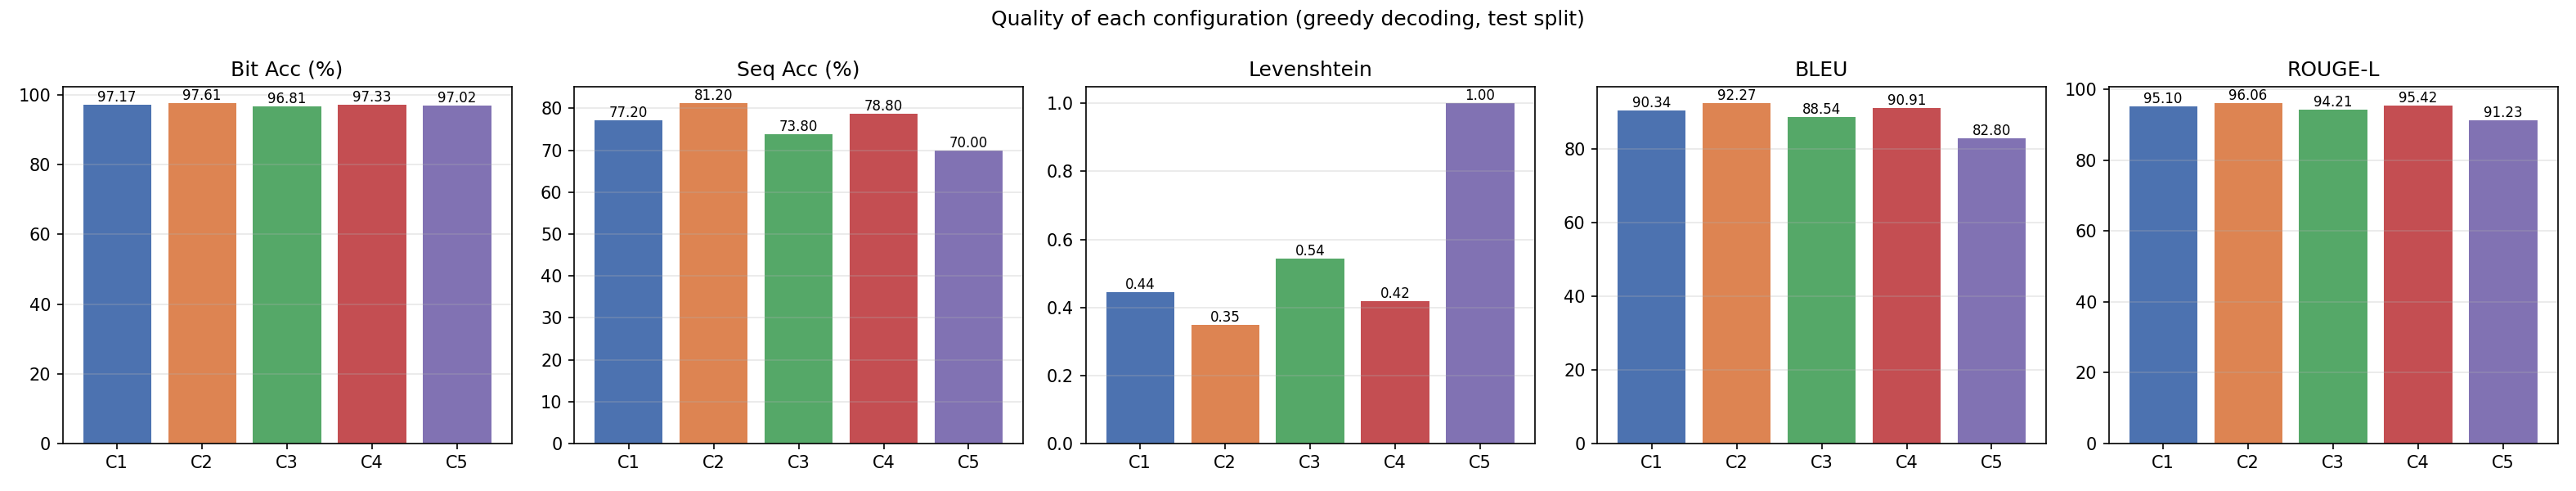
\includegraphics[width=\linewidth]{ablation_quality.png}
\caption{Decoding quality across the five configurations.}
\label{fig:quality}
\end{figure}

\subsection{C2: RoPE improves every quality metric for free}

Rotary embeddings give the largest gain among the tokenised models. Sequence
accuracy rises from \CfgOneSeq\% to \CfgTwoSeq\%, a \textbf{4.0-point absolute
improvement}, with bit accuracy \CfgTwoBit\%, edit distance \CfgTwoLev, and BLEU
up from \CfgOneBleu\ to \CfgTwoBleu. This costs \textbf{zero parameters}
(\CfgTwoPar\,M, identical to C1) and \textbf{zero extra memory} (\CfgTwoMem\,MB
against \CfgOneMem\,MB): RoPE adds no learnable weights, only a deterministic
rotation of $q$ and $k$.

This fits the task. By Eq.~\ref{eq:cipher} the output at position $i$ depends on
$i \bmod 8$, so the decoder needs not \emph{where} it is absolutely but \emph{how
far} it has advanced relative to the source it consumes, which is what RoPE
encodes: the logit is a function of the offset $m-n$ alone. The cost is
throughput, \CfgTwoSec\,s per epoch against \CfgOneSec\ (7.6\% slower); decoding
is unaffected, as the tables are precomputed.

\subsection{C3: GQA trades accuracy for parameters and decode speed}

GQA worsens every quality metric: sequence accuracy \CfgThreeSeq\% ($-3.4$
points), bit accuracy \CfgThreeBit\%, edit distance \CfgThreeLev. Collapsing 8
key/value heads to 2 removes \textbf{0.89\,M parameters} ($-11.6$\%) and forces
four query heads to share one key/value subspace, so the model represents fewer
distinct ways of matching queries against keys. Where the decoder must attend to
a precisely located 8-bit window, that lost specificity is not free. What GQA
buys is inference cost: decoding drops to \CfgThreeGen\,s ($-7.6$\%) and peak
memory to \CfgThreeMem\,MB, as the KV-cache shrinks fourfold.

One detail is easy to misread: C3 is \emph{slower} to train than C1
(\CfgThreeSec\ against \CfgOneSec\,s per epoch) despite having fewer parameters.
Under teacher forcing there is no KV-cache to shrink, so only the broadcast of 2
key/value heads back to 8 remains, which is pure overhead. GQA is an
\emph{inference-time} optimisation, and this experiment separates the two regimes.

\subsection{C4: RMSNorm is a strict improvement}

RMSNorm improves quality \emph{and} reduces cost on every axis at once. Sequence
accuracy rises to \CfgFourSeq\% ($+1.6$ over C1) and bit accuracy to
\CfgFourBit\%, while epoch time falls to \CfgFourSec\,s (7.7\% faster, quickest
of all five), peak memory to \CfgFourMem\,MB ($-6.0$\%), and decoding to
\CfgFourGen\,s ($-14.9$\%). Dropping mean-subtraction removes a full reduction
over the feature axis in both passes, and dropping the bias explains the small
parameter difference. The accuracy gap is within run-to-run noise (perplexities
\CfgFourPpl\ and \CfgOnePpl), so the honest reading is not ``RMSNorm is more
accurate'' but ``\textbf{re-centring contributes nothing measurable here, and its
cost is real}.'' Pre-norm streams are already approximately zero-mean.

% =====================================================================
\section{The token-free trade-off (C5)}
\label{sec:blt}

C5 is the only configuration that changes the input representation rather than a
computation inside the network, and the only one that loses to the baseline.
Sequence accuracy falls to \CfgFiveSeq\% against C1's \CfgOneSeq\%, a
\textbf{7.2-point drop}, edit distance more than doubles to \CfgFiveLev, and BLEU
falls to \CfgFiveBleu, yet bit accuracy is essentially unchanged
(\CfgFiveBit\%). The model gets the bytes right and assembles them badly.

\paragraph{Right bytes, wrong places.} C5 has the \emph{lowest} teacher-forced
perplexity of all five (\CfgFivePpl\ against \CfgOnePpl) yet the worst sequence
accuracy: given the correct prefix the next byte is almost determined, but under
free-running decoding it is weakest, so the errors are about \emph{where} a byte
belongs rather than \emph{which} one. C5 turns \texttt{half of the Mi} into
\texttt{off hald the M}, the right characters reordered with an insertion pushing
the rest out of phase, and one such slip forfeits the segment.

\paragraph{Why entropy patching is a poor fit \emph{here}.} By
Eq.~\ref{eq:cipher} the task is byte-local and rigidly aligned: after packing,
output byte $i$ depends on source byte $i$ and on $i \bmod 8$, so the ideal model
learns a fixed diagonal correspondence. Entropy patching is instead
\emph{content}-driven, and the two sides are cut at unrelated places: cipher
bytes are near-uniform ($H_0 = 6.04$ bits, threshold 4.94) so their boundaries
are near-arbitrary, while plaintext is English ($H_0 = 4.34$, threshold 3.98) and
breaks at word-like positions. Neither respects the key period of 8 nor aligns
with the other, so the bottleneck must rebuild a strict one-to-one correspondence
across boundaries that do not correspond. This reflects the interaction between
mechanism and task, not a defect of the mechanism: on natural language the same
procedure is what makes BLT work.

\paragraph{Cost.} Packing the bits makes the stream 32 bytes rather than 256, and
entropy patching compresses that to about 10.3 patches, so C5's global
transformer runs on a \emph{shorter} sequence than C1's 23 BPE tokens. Peak memory
is nevertheless \CfgFiveMem\,MB against \CfgOneMem\,MB ($1.41\times$): the saving
is outweighed by the byte-level periphery, two extra local stacks over the
34-byte stream plus the dense masks variable-length pooling needs. Epoch time is
\CfgFiveSec\,s ($1.93\times$) and decoding \CfgFiveGen\,s ($4.15\times$), as 32
bytes are emitted one at a time instead of roughly 21 tokens. The one clear win is
size: C5 has the \textbf{fewest parameters} (\CfgFivePar\,M), since dropping the
vocabulary deletes two $4096 \times 256$ embedding matrices.

% =====================================================================
\section{Conclusion}

\textbf{RoPE} buys $+4.0$ points of sequence accuracy for no parameters and no
memory; \textbf{GQA} costs 3.4 points and is \emph{slower} to train, its benefit
being a KV-cache effect teacher forcing never exercises; \textbf{RMSNorm} is free
on every axis; and the \textbf{token-free BLT} costs 7.2 points at $1.41\times$
memory and $4.15\times$ decode time, with the fewest parameters. \looseness=-1
The three changes \emph{inside} the network are small and roughly free, while the
change to the \emph{representation} dominates, its sign depending on whether it
respects the mapping's structure. BPE merges cut across the byte boundaries this
cipher is defined on, so C1 makes substitution errors; entropy patches cut the
sides at unrelated positions, so C5 makes positional ones. A representation is
good or bad only relative to the alignment a task demands.


% =====================================================================
\section*{Links}
\addcontentsline{toc}{section}{Links}

\begin{itemize}\itemsep1pt
\item \textbf{Weights \& Biases project (all five runs):}\\
      \url{https://wandb.ai/vidvathama-babu-iiit-hyderabad/anlp-a1-blt-ablation}
\item \textbf{Hugging Face checkpoints (C1--C5):}\\
      \url{https://huggingface.co/Viv0605101/anlp-a1-transformer-blt-ablation}
\end{itemize}

% =====================================================================
\bibliographystyle{plainnat}
\bibliography{refs}

\end{document}
